\chapter{Software Design Overview}
{
    \renewcommand*{\theenumi}{\thesubsection.\arabic{enumi}}
    \renewcommand*{\theenumii}{\theenumi.\arabic{enumii}}
    \renewcommand*{\theenumiii}{\theenumii.\arabic{enumiii}}

    \section{Description}

        The DRINC project uses various pieces of software to control the 
        pouring mechanisms and front end features. the DRINC project will 
        consist of the following pieces of software:
        \begin{itemize}
            \item The microprocessor code
            \item The server code to communicate with the drink flow
            \item The server code to present the API
            \item The client code to render the display for the user
        \end{itemize}
        The microprocessor code is documented in the hardware section.

    \section{Display Backend}
        The generalplan for the backend is to write modules in PHP. These 
        modules will either be running in the background and communicating 
        data to and from the database through means of an API. 

        PHP will allow the ease of use in communication between the PHP and 
        PostgreSQL database by use of sanitized Structured Query Language (
        SQL) queries and ability to escape all output. This will eliminate 
        the chances of SQL injection (SQLi) and Cross-site scripting (XSS) 
        attacks on the system.

    \section{Display Frontend}
        The front end will be displayed using mainly HTML, with some PHP and 
        Javascript for anything dynamic. The frontend will communicate with 
        the backend using API.

    \section{Program Flow}
        This program will have three main ``threads''. One thread would be 
        responsible for listening to user input coming from the Android 
        tablet and another would be responsible for communicating with the 
        Arduino device controlling the dispensary of fluids. The last thread 
        will be responsible for communicating with the database and 
        receiving or adding data.

        The user input thread will be responsible for receiving all input 
        via Android tablet or the website. It will communicate with the API 
        which will inturn communicate with either the database or fluid 
        dispensary thread when needed. Therefore, all this thread needs to 
        do is listen for user commands and send the processed commands to 
            the correct thread.

        The Arduino thread will be responsible for communicating to the 
        Arduino device controlling the fluid dispensary. It will take input 
        from the API, originating from the input thread, and control the 
        fluid flow as such. When a user request is handled and the drink 
        recipe is collected via the other threads, a listing of array 
        positionings and the amount for each will be passed to the arduino 
        using this thread.

        The database thread will be responsible for communicating with the 
        database. Its job will be to lookup things in the database along 
        with inputting/changing/deleting things. The things consists of: 
        types of base drinks, recipes for mixed drinks, and the current 
        positioning of the currently loaded drinks. It will receive its 
        information, along with forward responses, to/from the API.

    \section{Data Flow}
        The applications will use PostgreSQL to store all of the data. Both 
        the website and the Android app will be able to access the 
        information in the database via an API, which will interact with the 
        database as needed for the applications.

        \begin{figure}[htb]
            \centering
            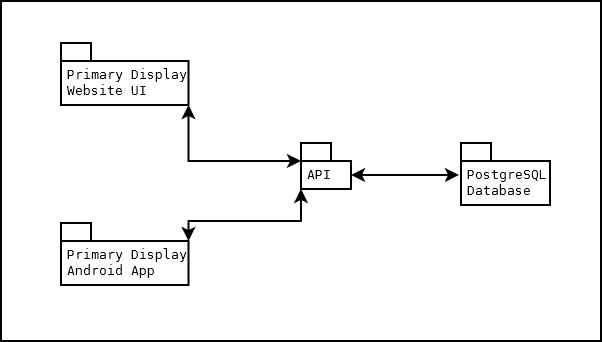
\includegraphics[width=0.9\textwidth]{Images/DataFlow.png}
            \caption{Diagram of Data Flow}
            \label{fig:DataFlow}
        \end{figure}

    \section{Potential Problems}
        One potential problem is that their is a limited time constraint. 
        Since we will be working with different technologies and languages 
        that we have not currently worked with, a bulk of our time will be 
        used by learning such.

    \section{The Backend}

        \subsection{Authentication}
            The authentication module will be used every time a user attempts to 
            log in. This module will use the user commands thread to communicate 
            with the API. It will send the login information given by the user 
            to the API, in which the API will check to see if the user 
            information is valid. If it is, the API will tell the module to log 
            the user in. Otherwise, it will tell the module to deny the login 
            attempt and print an error.

        \subsection{API}
            The API will deal with all of the backend communication between the 
            website/Android app and the server. This includes authentication, 
            deleting a drink from the user's list, adding a drink to the user's 
            list and requesting access to the drinks in the user’s list when the 
            user wishes to create a drink.

}
